\documentclass[12pt]{article}
\usepackage[a4paper, total={6in, 8in}]{geometry}
\usepackage[utf8]{inputenc}
\usepackage{booktabs}
\usepackage{rotating}
\usepackage{multirow}
\usepackage[graphicx]{realboxes}
\usepackage{stackengine}
\usepackage{epigraph}
\usepackage{float}
\usepackage{dcolumn}
% \usepackage{longtable}
\usepackage{supertabular}
% \usepackage[nomarkers]{endfloat}
\usepackage{acronym}
\usepackage{listings}
\usepackage{hyperref}
\hypersetup{colorlinks=true,%
citecolor=black,%
filecolor=black,%
linkcolor=black,%
urlcolor=black
}
\usepackage[portuguese]{babel}
\usepackage[autostyle,portuguese=brazilian]{csquotes}
\usepackage{setspace} % for \onehalfspacing and \singlespacing macros
\onehalfspacing
\usepackage{etoolbox}
\usepackage{amsmath}
\AtBeginEnvironment{quote}{\singlespacing\small}
% \usepackage[usestackEOL]{stackengine}
\usepackage[justification=centering]{caption}
\usepackage[notes,backend=biber]{biblatex-chicago}
\usepackage{subfig} %incluir Figura side by side
%codigo  para spacing 1.5
%\usepackage{setspace}
%\doublespacing
%codigo para monospace justificado tt
\renewcommand{\familydefault}{\rmdefault}
%codigo estilo dos numeros
\usepackage[sc,osf]{mathpazo}
\usepackage{ragged2e}
\justifying

\usepackage{listings}
\usepackage{xcolor}

\definecolor{codegreen}{rgb}{0,0.6,0}
\definecolor{codegray}{rgb}{0.5,0.5,0.5}
\definecolor{codepurple}{rgb}{0.58,0,0.82}
\definecolor{backcolour}{rgb}{0.95,0.95,0.92}

\lstdefinestyle{mystyle}{
    backgroundcolor=\color{backcolour},   
    commentstyle=\color{codegreen},
    keywordstyle=\color{magenta},
    numberstyle=\tiny\color{codegray},
    stringstyle=\color{codepurple},
    basicstyle=\ttfamily\footnotesize,
    breakatwhitespace=false,         
    breaklines=true,                 
    captionpos=b,                    
    keepspaces=true,                 
    numbers=left,                    
    numbersep=5pt,                  
    showspaces=false,                
    showstringspaces=false,
    showtabs=false,                  
    tabsize=2
}

\lstset{style=mystyle}

\bibliography{references.bib}

\usepackage{enumitem}
\newlist{floatnotes}{description}{1}
\setlist[floatnotes]{font=\normalfont\itshape,wide, nosep, leftmargin=.1\linewidth, itemindent=\labelsep, rightmargin=\leftmargin, before=\vspace{.5em}\footnotesize}

\usepackage{pdflscape}
\usepackage{afterpage}
\usepackage{capt-of}% or use the larger `caption` package
\usepackage{enumitem}

\makeatletter
%Add packages here
\usepackage{hyperref}

\begin{document} 

\newgeometry{margin = .65in, top=1.05in}
\linespread{1.1}

\title{%
  A mulher negra no mercado de trabalho brasileiro na última década: educação, representatividade e desigualdades salariais\\
  \vspace{1cm}
  \Large \texttt{\MakeUppercase{DRAFT}}}

\author{Pacto de Promoção da Equidade Racial \thanks{Responsáveis técnicos: Crislane Alves e Lucas Cavalcanti Rodrigues}}


\maketitle

\section{Fatos estilizados}

\par Nesta seção, apresentam-se fatos estilizados sobre a participação da população negra no mercado de trabalho brasileiro, com ênfase no sub-grupo demográfico representado pelas mulheres negras. Os fatos estilizados constituem-se em aspectos conhecidos sobre determinado tema de pesquisa e baseados na literatura e dados existentes. Para o tema sob análise, tem-se os seguintes fatos estilizados:

\begin{enumerate}
    \item Homens negros, mulheres brancas e mulheres negras têm salários médios inferiores a homens brancos.
    \item Considerando os 4 sub-grupos demográficos, os salários médios das mulheres negras são os mais baixos, seguidos pelos salários de homens negros, mulheres brancas e homens brancos.
    \item Entre 1987 e 2000, o \textit{gap} salarial entre mulheres negras e homens brancos diminuiu à taxa de 0,7\% ao ano. Enquanto para mulheres brancas essa redução foi de aproximadamente 1\% ao ano.
    \item Entre 1987 e 2000, o \textit{gap} salarial entre homens negros e homens brancos permaneceu constante.
\end{enumerate}

\par Os fatos estilizados apresentados acima são baseados na literatura existente.\footnote{Para os fatos estilizados de 1-4, ver \cite{soares2000perfil}} Embora esses fatos tenham o benefício de apresentar um quadro geral sobre as condições de participação da mulher negra no mercado de trabalho, a mera revisão da literatura existente falha em apresentar um quadro coeso e atualizado da situação da mulher negra no mercado de trabalho. Isso ocorre tanto em função de recortes temporais feitos por pesquisas mais antigas, quanto pelo foco escolhido por cada pesquisador no mercado de trabalho, seja formal ou informal. Com o objetivo de atualizar os dados apresentados pela literatura existente e abarcar tanto o mercado formal quanto o mercado informal de trabalho, esta seção apresenta dados atualizados dos fatos destacados pela literatura existente usando as duas principais bases administrativas do mercado de trabalho brasileiro, RAIS e PNAD.

\par Começa-se, assim, por avaliar o primeiro fato estilizado. As tabelas X e Y apresewntam, respectivamente, a média salarial de homens negros, mulheres brancas, mulheres negras e homens brancos usando dados da PNAD e RAIS. O dado da PNAD é mais atualizado e refere-se ao trimestre X de 2022, enquanto o dado da RAIS refere-se estritamente ao mercado formal de trabalho e cobre o ano de 2020.




\section{O IEER de mulheres negras} 


\par Os resultados apresentados nesta minuta referem-se a indicadores de representação, salário e oferta de trabalho de mulheres negras no mercado formal brasileiro entre 2010 e 2020. Os dados e a discussão são feitos em uma perspectiva comparada considerando, assim, outros sub-grupos demográficos como homens negros, e homens e mulheres brancos.

\par O primeiro resultado apresentado é o IEER atual das mulheres negras no mercado de trabalho forma brasileiro. Antes de apresentar os resultados, porém, é importante destacar uma questão relacionada à interpretação do IEER. O IEER, originalmente, mensura o número de desvios padrões em que o número de negros em determinada ocupação supera o valor esperado de negros dado uma população de referência. Esse valor, contudo, passa por uma transformação algébrica, com o objetivo de comparar o índice entre diferentes ocupações e empresas e fixar seu intervalo em [-1,1]. A transformação algébrica viabiliza a interpretação relativa, ao custo de limitar a possibilidade de interpretação absoluta do índice. Por essa razão, o valor do índice não pode ser interpretado em termos absolutos e, em particular, não tem uma interpretação de \enquote{elasticidade}. Um setor, por exemplo, com IEER=-0,32 não tem 32\% a menos de negros do que seria esperado. Esta é uma interpretação errada.

\par Por outro lado, a magnitude do valor absoluto do índice mostra sim \textit{o grau} de sub ou sobre-representação de negros na unidade produtiva. Assim, por exemplo, um empresa com IEER=-0.8 tem uma desigualdade racial nas suas ocupações \textit{maior} que uma empresa com IEER=-0.6. Para ajudar na interpretação dos valores do IEER, os autores do índice de equidade ocupacional, que serve de base para o IEER, sugeriram a seguinte classificação.\autocite{ransom2001one}

\begin{table}[htb!]
\centering
\caption{Interpretação dos intervalos do Índice ESG de Equidade Racial}
\begin{tabular}{lc}
\hline
Grupo             & Intervalo                 \\ \hline
Não-Mulher Negra Excluídos & $IEER \geq 0, 8 $               \\
Dominância Mulher Negra  & $0,2 < IEER < 0,8$   \\
Equidade          & $-0,2\leq IEER \leq 0,2$  \\
Dominância Não-Mulher Negra & $-0,8 < IEER < -0,2$ \\
Mulher Negra Excluída  & $IEER \leq -0,8$        \\ \hline
\end{tabular}
\end{table}

\par Os valores apresentados na tabela \ref{tab:ieer_2020} mostram, então, que mulheres negras estão sub-representadas no mercado de trabalho formal brasileiro em uma proporção em que é possível falar em \textit{dominância} dos demais grupos demográficos, mas não \textit{exclusão} de mulheres negras. Chega-se a essa interpretação ao se observar o valor do IEER Ponderado, principal indicador na tabela \ref{tab:ieer_2020}. Os demais IEERs mostram a situação de representatividade de mulheres negras em 3 grupos de ocupação, não-liderança, gerência e diretoria. Fica claro que a representação de mulheres negras é maior em ocupações de não-liderança e diminui a medida que se avança no nível hierárquico das ocupações. Os resultados da tabela \ref{tab:ieer_2020} referem-se a trabalhadores formais de todas as empresas brasileiras em 2020. É possível que os resultados observados variem quando se considera heterogeneidades regionais e econômicas das empresas.

\begin{table}[htb!]
    \centering
    \small
    \caption{Índice ESG de Equidade Racial - Mulheres Negras - 2020}
    \begin{tabular}{lc}
    \hline
    \multicolumn{1}{c}{Grupo} & IEER   \\ \hline
    Não-Liderança             & -0.579 \\
    Gerência                  & -0.656 \\
    Diretoria                 & -0.760 \\
    Ponderado                 & -0.665 \\ \hline
    \end{tabular}
    \label{tab:ieer_2020}
    \begin{floatnotes}
    \item [Fonte:] RAIS 2020.
    \item [Nota:] A população de referência utilizada é igual à metade da população de pretos e pardos.
    \end{floatnotes}
    \end{table}

\par Como a situação de representatividade da mulher negra de hoje se compara com a última década? Esta pergunta é respondida pela figura \ref{fig:ieer_evolution} que apresenta a evolução do IEER Ponderado e dos IEERs ocupacionais de 2010 a 2020. Fica evidente que há uma evolução favorável no sentido de aumento da representação de mulheres negras nos últimos 10 anos. O resultado, que aparece no IEER Ponderado, é consequência da evolução favorável dos 3 IEERs ocupacionais, inclusive diretoria. Em que pese o fato da sub-representação de mulheres negras ser ainda muito elevada em 2020, como visto na tabela \ref{tab:ieer_2020}.

\begin{figure}[H]
    \centering
    \caption{Evolução do IEER Ponderado - Mulheres Negras - 2010/2020}
        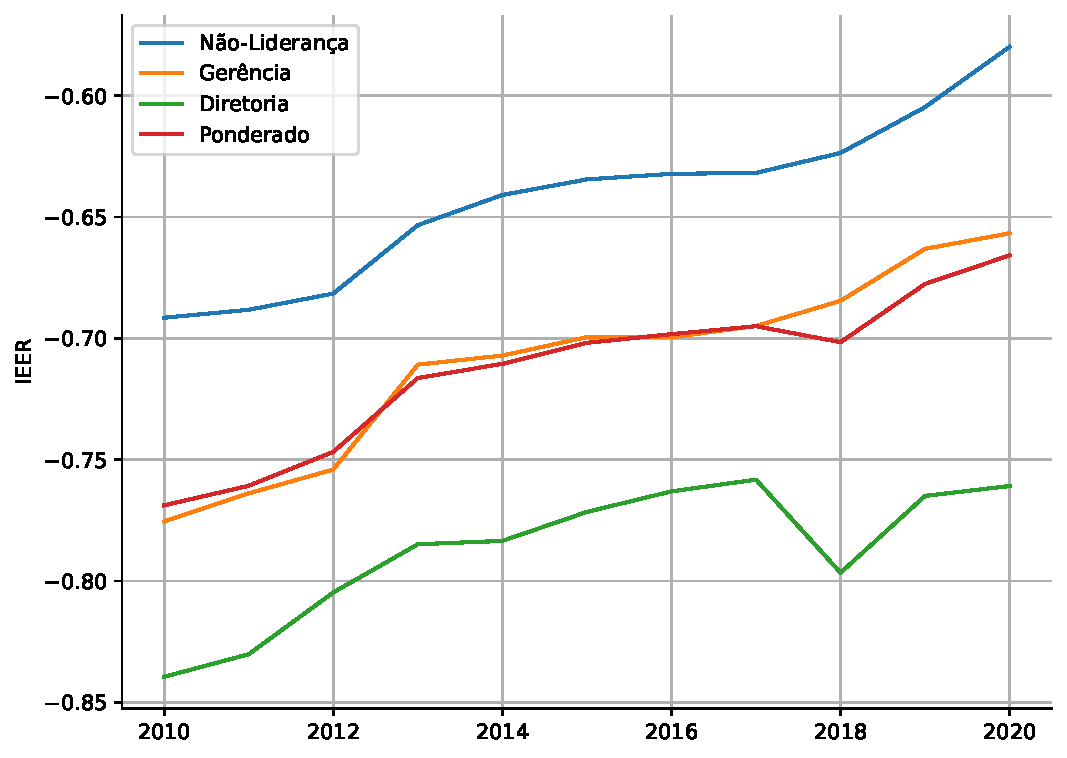
\includegraphics[height=8cm]{/home/dell/Documents/pacto/reports/black_women/figures/ieer_black_women.pdf}
    \label{fig:ieer_evolution}
\end{figure}

\par O IEER é uma medida de representatividade que leva em conta a desigualdade salarial. Isto porque o indicador de desigualdade ocupacional que serve de base para o IEER é ponderado pela massa salarial, dando maior peso a ocupações com maior nível salarial. Dessa forma, seria possível que parte da melhora observada na figura \ref{fig:ieer_evolution} fosse causada pela queda da desigualdade salarial no período. A figura \ref{fig:wage_gap} mostra, porém, que este não é o caso. Na figura, observa-se a evolução da proporção do salário de homens negros, mulheres brancas e mulheres negras em relação ao salário de homens brancos. Fica claro a estagnação dos salários relativos de mulheres negras que, no período, perceberam aproximadamente 55\% do salário recebidos por homens brancos.

\begin{figure}[H]
    \centering
    \caption{Evolução do IEER Ponderado - Mulheres Negras - 2010/2020}
        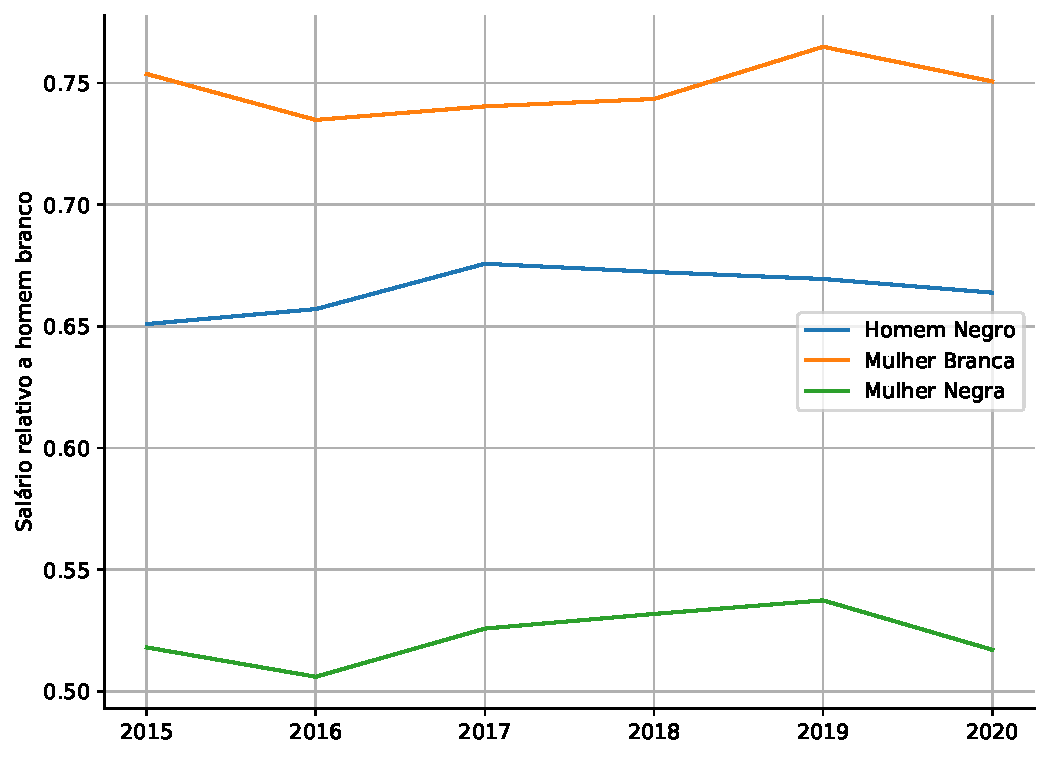
\includegraphics[height=8cm]{/home/dell/Documents/pacto/reports/black_women/figures/wage_gap.pdf}
    \label{fig:wage_gap}
\end{figure}

\par A figura \ref{fig:supply_gap} mostra que, de fato, a provável explicação da melhora do IEER das mulheres negras na última década esteja no aumento do quantitativo de trabalhadores negros no mercado de trabalho formal no período. A figura que, em relação a homens brancos, o número de mulheres negras com carteira assinada avançou cerca de 30 pontos percentuais, saindo de aproximadamente 30\% em 2010 e alcançando pouco mais de 50\% em 2020.


\begin{figure}[H]
    \centering
    \caption{Evolução do IEER Ponderado - Mulheres Negras - 2010/2020}
        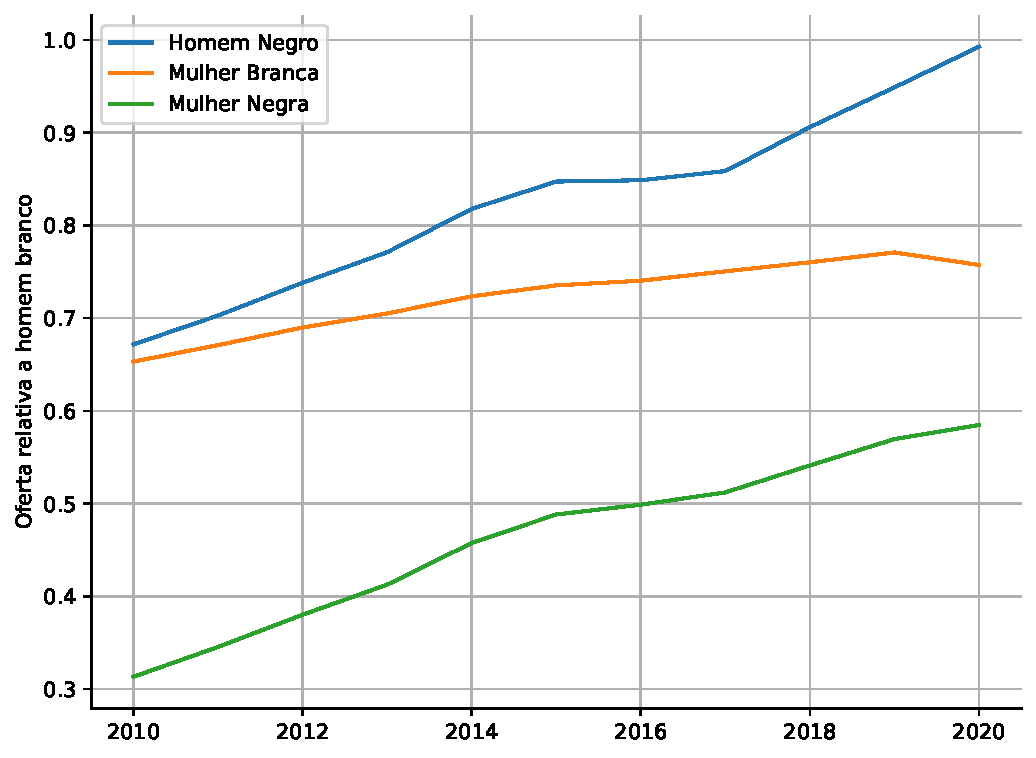
\includegraphics[height=8cm]{/home/dell/Documents/pacto/reports/black_women/figures/supply_gap.pdf}
    \label{fig:supply_gap}
\end{figure}

\begin{table}
\centering
\caption{Composição educacional da oferta de trabalho de mulheres negras - 2010-2020}
\begin{tabular}{lrrr}
\toprule
{} &  Até Fundamental &  Ensino Médio &  Superior+ \\
ano  &                  &               &            \\
\midrule
2010 &            23.9\% &         63.1\% &      13.0\% \\
2011 &            22.4\% &         64.5\% &      13.1\% \\
2012 &            21.3\% &         65.3\% &      13.4\% \\
2013 &            20.2\% &         65.9\% &      14.0\% \\
2014 &            18.5\% &         66.5\% &      15.0\% \\
2015 &            17.7\% &         66.6\% &      15.8\% \\
2016 &            16.3\% &         66.0\% &      17.7\% \\
2017 &            15.0\% &         66.3\% &      18.7\% \\
2018 &            14.0\% &         65.8\% &      20.1\% \\
2019 &            13.2\% &         66.4\% &      20.4\% \\
2020 &            12.4\% &         66.8\% &      20.8\% \\
\bottomrule
\end{tabular}
\end{table}


\begin{figure}[H]
    \centering
    \caption{Evolução do IEER Ponderado - Mulheres Negras - 2010/2020}
        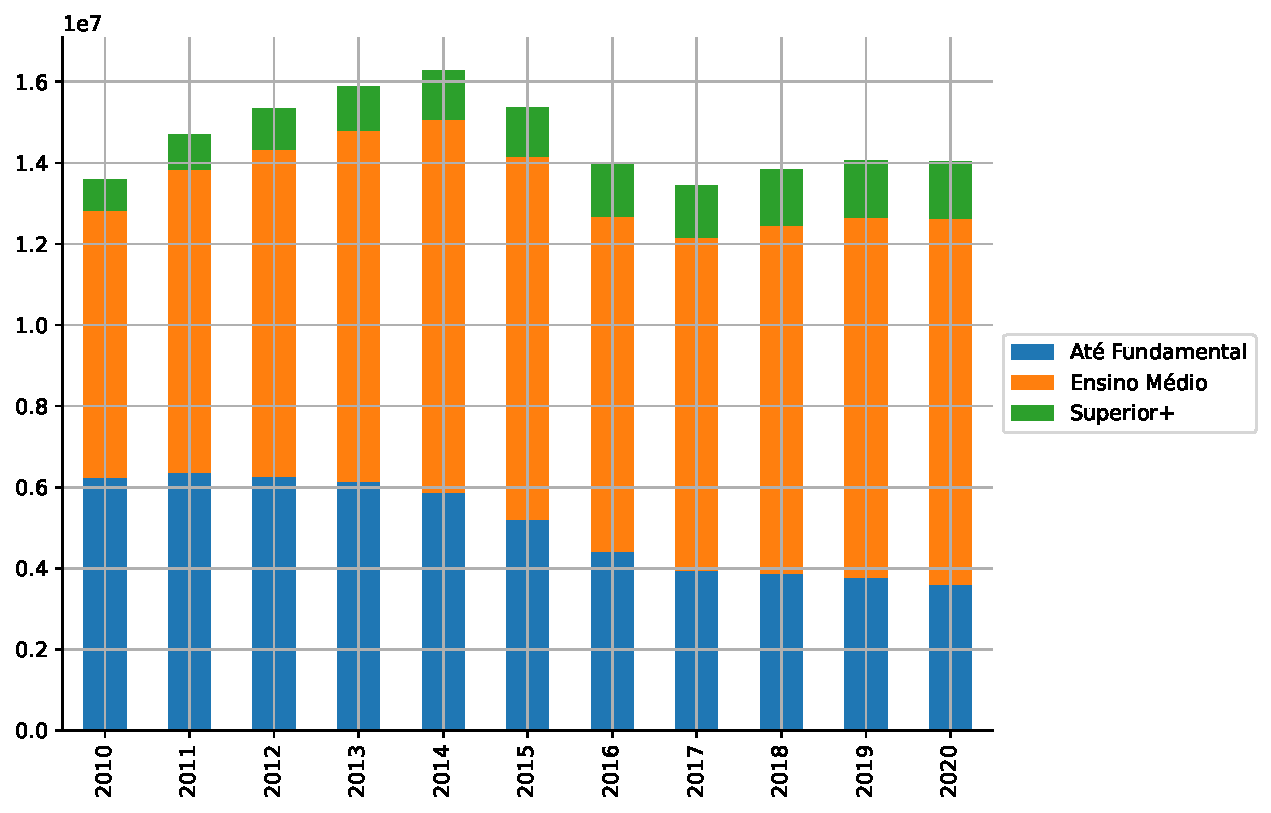
\includegraphics[height=8cm]{/home/dell/Documents/pacto/reports/black_women/figures/education_main_groups.pdf}
    % \label{fig:ieer_evolution}
\end{figure}

\clearpage

\printbibliography[title={Bibliografia}, nottype=misc]

\end{document}